\section{DIP platforma}

Izstrādātā platforma sastāv no \glslink{server}{servera}, \glslink{agent}{aģentiem}
jeb aparatūras starpniekiem, pašas fiziskās attīstītājrīku aparatūras,
\glslink{client}{klientiem} jeb gala lietotājiem ar komandrindas rīkiem, un
pārvaldības paneļa jeb datu pārvaldības tīmekļa lietotnes. Attēlā
\ref{fig:dipdpd0} redzama 0. līm. datu plūsmas diagramma minētai platformai. 

\begin{figure}[H]
    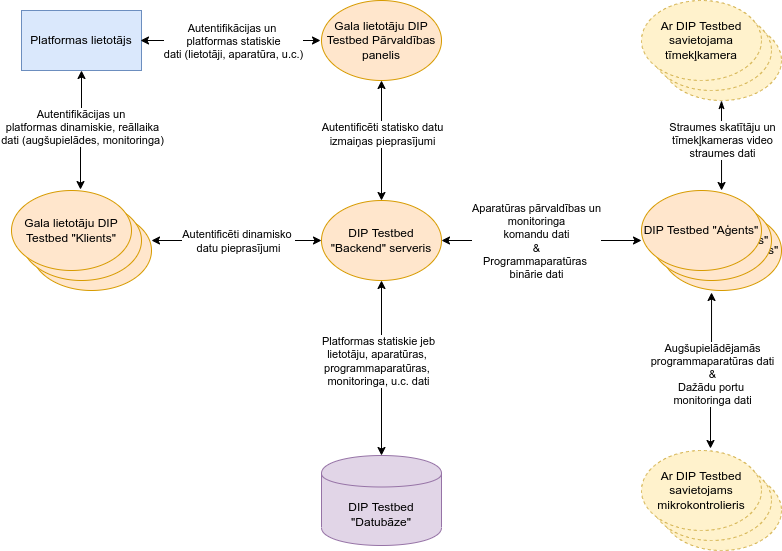
\includegraphics[width=0.7\linewidth]{assets/DPD0.drawio.png}
    \centering
    \caption{DIP platformas 0. līmeņa datu plūsmas diagramma}
    \label{fig:dipdpd0}
\end{figure}

Attēlā \ref{fig:dipdpd0} redzamās apakšsistēmas ir aprakstītas šajā dokumentā
sekojoši. 

Pašā platformas centrā ir centralizēts tīmekļa serveris, kas funkcionē
kā pārvaldības datu avots un platformas lietotāju komunikācijas starpnieks, tā
datu pārvaldības ir aprakstīta nodaļās \ref{sec:usermgmt} un \ref{sec:hwmgmt},
savukārt, tā dalība komunikācijas mehānismos ir aprakstīta \ref{sec:dipactorsystem}.

Nodaļā \ref{sec:dipactorsystem} aprakstītā vājo reāllaika komunikācijas sistēmu,
savukārt, izmanto komandrindas rīki - klients un aģents - lai ļautu lietotājiem
mijiedarboties ar attīstītājrīku aparatūru. Šis mehānisms ir aprakstīts nodaļā
\ref{sec:agentclient}. Un izmantojot šo klienta - aģenta mehānismu, platformā
lietotājam tiek realizētas trīs saskarnes, lai mijiedarbotos ar attīstītājrīku
aparatūru, kuras aprakstītas nodaļās \ref{sec:vinweb}, \ref{sec:vinbytes} un
\ref{sec:vinminos}.

Par šīs platformas, tai skaitā aparatūras laboratoriju, uzstādīšanu un
administrēšanu ir aprakstīts nodaļā \ref{sec:ops}. Par programmaparatūras
izstrādi un testēšanu platformā mazliet aprakstīts nodaļā \ref{sec:usage}. Par
šī darba veikumu un tvērumu aprakstīts nākamajā nodaļā \ref{sec:scope}.

\section{Darba tvērums}
\label{sec:scope}

Darba ietvaros tika izstrādāta vāja reāllaika komunikācijas platforma, kas
nodrošina 1) iespēju reģistrēt un uzskaitīt, pārvaldīt fizisku attīstītājrīku
vai mikrokontrolieru aparatūru, 2) veikt programmaparatūras augšupielādi
aparatūrā, 3) mijiedarboties ar aparatūru, izmantojot vizuālu saskarni, kas
līdzinās noklusētajai aparatūrā fiziski pieejamajai saskarnei, 4) ierobežoti
testēt aparatūras funkcionalitāti. Papildus platforma tika arī testēšanas
nolūkiem izveidota publiskā mākoņpakalpojumu serverī, kas aprakstīts avota koda
repozitorijā un nodaļā \ref{sec:ops}. \cite{VeinbahsKrisjanisTestbed}
\cite{VeinbahsKrisjanisProduction}

Šis darbs izstrādāts atvērti - platformas pirmkods un šī dokumenta pirmkods ir
publiski pieejams GitHub platformā brīvai apskatei un izmantošanai.
\cite{VeinbahsKrisjanisTestbed} \cite{VeinbahsKrisjanisThesis}.

\begin{table}[H]
    \begin{tabular}{ |p{3cm}|p{3cm}|p{3cm}|p{3cm}|p{3cm}| }
    \hline
    Programmēšanas valoda&Faili&Tukšās rindiņas&Komentāru rindiņas&Koda rindiņas\\
    \hline
    Python & 101 & 1551 & 717 & 7424\\
    Scala & 101 & 593 & 120 & 4088\\
    Verilog & 34 & 409 & 676 & 2496\\
    HTML & 11 & 3 & 0 & 492\\
    Bourne Shell & 17 & 91 & 85 & 378\\
    make & 2 & 36 & 30 & 80\\
    SQL & 2 & 33 & 28 & 70\\
    XML & 1 & 14 & 8 & 40\\
    YAML & 2 & 0 & 1 & 33\\
    C++ & 1 & 4 & 14 & 14\\
    \hhline{|=|=|=|=|=|}
    Kopā & 272 & 2734 & 1679 & 15115\\
    \hline
    \end{tabular}
    \centering
    \captionsetup{justification=centering}
    \caption{Koda rindiņu skaita analīze projekta pirmkodā}
    \label{table:cloc}
\end{table}

Aptuvenai sapratnei par izstrādāto koda apjomu, projekta pirmkodā tika izpildīts
koda rindiņu analīzes rīks \cite{AlDanialCloc}, kura rezultāti redzami gan projekta
pirmkoda versiju kontroles repozitorijā \cite{VeinbahsKrisjanisTestbed}, gan tabulā
\ref{table:cloc}.

Platformas pamata funkcionalitāte, lai lietotājs augšupielādētu programmatūru un
veiktu baitu līmeņa datu apmaiņu ar aparatūru, tika realizēta kursa darba laikā.

Bakalaura darba laikā, 1) platformai tika pievienota autentifikācija, 2)
izstrādāts pārvaldības panelis, 3) pārrakstīts klients no tīras grafiskas
saskarnes par termināļa grafisko saskarni, 4) pārrakstīta klienta virtuālā
saskarne kā notikumu sistēma nevis nestrukturizēts kods, 5) izplānota un
realizēta virtuālā saskarne MinOS formālā protokolā, klientā un attīstītājrīkā,
6) tika dokumentēta sistēmas darbība un arhitektūra, tai skaitā arī šī dokumenta
izstrāde.

\section{Statisko datu pārvaldība}
\label{sec:staticdata}

Šī platforma pamatā sastāv no reāllaika datu starpniecības un statisku datu
pārvaldības. Par statiskajiem datiem tiek uzskatīti tādi dati, kurus lietotājs
nemaina izmantojot vājā reāllaika komunikācijas kanālus, kas aprakstīti sadaļā
\ref{sec:dipactorsystem}. 

\begin{figure}[H]
    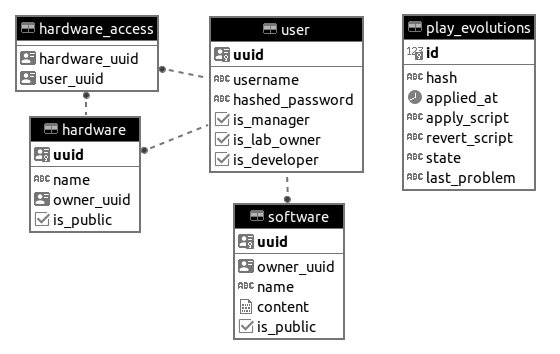
\includegraphics[width=0.7\linewidth]{assets/physical-er-diagram-gray.png}
    \centering
    \caption{Platformas fiziskā līmeņa datubāzes relāciju diagramma.}
    \label{fig:staticdata}
\end{figure}

Attēlā \ref{fig:staticdata} redzama platformas izstrādes laikā izveidotā
datubāzes fiziskā līmeņa relāciju diagramma, kurā redzamas tabulas lietotājiem
\lstinline!user!, programmaparatūrai \lstinline!software!, aparatūrai
\lstinline!hardware! un aparatūras piekļuvei \lstinline!hardware_access!, kā arī
papildus tabula datubāzes migrāciju vēstures pārvaldībai
\lstinline!play_evolutions!, kas ir noklusēts tabulas nosaukums projektā
izmantotajam Scala programmēšanas valodas tīmekļa lapu izstrādes ietvaram "Play
Framework".

Lielākoties visām biznesa loģikas entītijām ir piesaistīts \gls{uuid}
identifikators \lstinline!uuid! un nosaukums \lstinline!name!, papildus dažām
entītijām ir dažādi piekļuves dati formātā \lstinline!is_*!, programmaparatūrai
ir arī tās saturs \lstinline!content! un lietotājam ir paroles ar jaucējvērtību
datiem \lstinline!hashed_password!.

Programmaparatūras tabulu varētu arī saukt \lstinline!firmware!, taču platformas
izstrādes laikā tika eksperimentēts platformā arī reģistrēt ne tikai
attīstītājrīku aparatūru, bet arī programmējamus mikrokontrolierus, kuros
augšupielādē programmatūru.

Darba ietvaros tika arī apsvērta tabula \lstinline!hardware_messages!, lai
glabātu vēsturi par notikušo vājā reāllaika komunikāciju, taču laika
ierobežojumu dēļ šī funkcionalitāte netika realizēta, jo nebija kritiska
platformas funkcionētspējai.

\section{Lietotāju datu pārvaldība}
\label{sec:usermgmt}

Lietotāju uzskaitei izmantota attēlā \ref{fig:staticdata} redzamā tabula
\lstinline!user!. Lietotājam ir iespējamas trīs iespējamas lomas pārvaldnieks
\lstinline!manager!, laboratorijas īpašnieks \lstinline!lab_owner! un
izstrādātājs \lstinline!developer!, atkarībā no kuras lietotājam platforma
piedēvē attiecīgas tiesības veikt dažādas darbības, kuras skatāmas tabulā
\ref{table:permissions}.

\begin{table}[H]
    \newcounter{permissioncounter}
    \newcommand\rownumber{\stepcounter{permissioncounter}\arabic{permissioncounter}.}
    \begin{tabular}{ |p{1cm}|p{5cm}|p{3cm}|p{6cm}| }
    \hline
    N.p.k.&Darbība&Nepieciešamās tiesības&Papildus nosacījumi \\
    \hline
    \rownumber & Lietotāja bez tiesībām izveide & - & Lietotājvārds nevar būt aizņemts \\
    \hline
    \rownumber & Lietotāju datu uzskaite & \lstinline!is_manager! vai \lstinline!is_lab_owner! & Jebkurš var lasīt savus datus \\
    \hline
    \rownumber & Lietotāja tiesību maiņa & \lstinline!is_manager! & - \\
    \hline
    \rownumber & Programmaparatūras augšupielāde & \lstinline!is_developer! & - \\
    \hline
    \rownumber & Programmaparatūras piekļuve & \lstinline!is_developer! vai
        \lstinline!is_manager! & Jebkurš var lasīt savu vai publicētu
        (\lstinline!is_public!) programmaparatūru \\
    \hline
    \rownumber & Programmaparatūras publicēšana & \lstinline!is_manager! & - \\
    \hline
    \rownumber & Aparatūras izveide & \lstinline!is_lab_owner! & - \\
    \hline
    \rownumber & Aparatūras publicēšana & \lstinline!is_manager! vai
        \lstinline!is_lab_owner! & Pārvaldnieks var publicēt visu, citi tikai
        savu \\
    \hline
    \rownumber & Aparatūras uzskaite & \lstinline!is_manager! vai
        \lstinline!is_developer!, vai \lstinline!is_lab_owner! & Pārvaldnieks
        var uzskaitīt visu, citi tikai savu vai \lstinline!hardware_access!
        tabulā piesaistīto \\
    \hline
    \rownumber & Aparatūras tiesību maiņa & \lstinline!is_manager! vai
        \lstinline!is_developer!, vai \lstinline!is_lab_owner! & Pārvaldnieks
        var pārvaldīt visu, citi tikai savu \\
    \hline
    \end{tabular}
    \centering
    \captionsetup{justification=centering}
    \caption{Lietotāju tiesības un pieejamās darbības}
    \label{table:permissions}
\end{table}

Platformā projekta programmatūras konfigurācijā ir konfigurējams administratora
lietotājs ar visām trīs iepriekšminētajām tiesībām, lai izveidotu sākotnējos
pārvaldības lietotājus.

Platformā lietotājus un to piekļuves datus var konfigurēt no
\glslink{mgmtpanel}{pārvaldības paneļa}, kas ir atšķirīgi no pārējām platformas
darbībām, kas lielākoties norit komandu rindā jeb terminālī, jo šos datus
pārsvarā pārvalda pasniedzējs vai laboratorijas īpašnieks, kuram visvieglāk būtu
no jebkura datora atvērt pārlūku un veikt šīs darbības. Savukārt, izstrādātājam,
kas pārsvarā savu darbu veic komandurindā, lielākā daļa darbības ir pieejamas
izmantojot komandu rindas rīku jeb \glslink{client}{klientu}. Skats no
pārvaldības paneļa lietotāju sadaļas skatāms attēlā \ref{fig:mgmtpanelusr}.

\begin{figure}[H]
    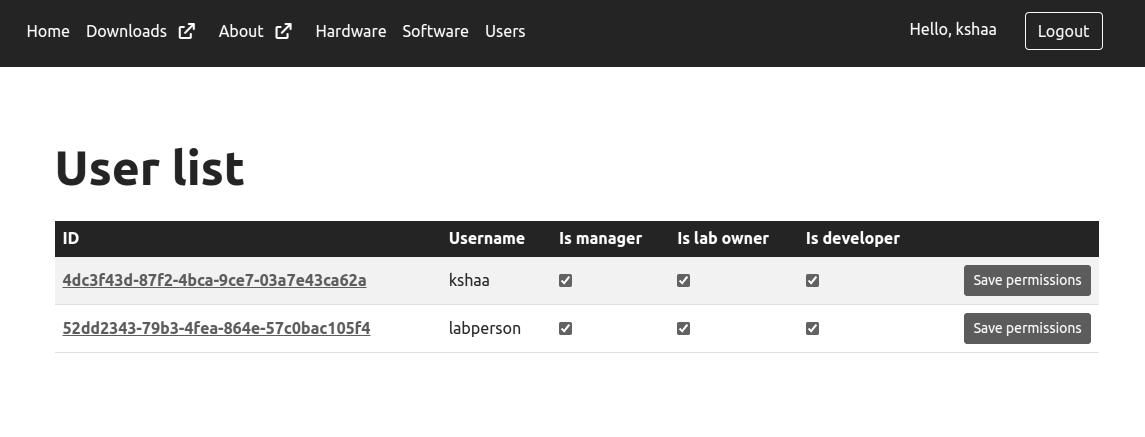
\includegraphics[width=0.9\linewidth]{assets/mgmt-panel-usr-gray.png}
    \centering
    \caption{Platformas pārvaldības paneļa lietotāju pārvaldības skats.}
    \label{fig:mgmtpanelusr}
\end{figure}

\section{Notikumu sistēmu realizācija}
\label{sec:dipactorsystem}

Darbā izstrādātajā platformā, lai veiktu ziņu starpniecību starp lietotāju un
aparatūru, bija nepieciešams realizēt vāja reāllaika komunikāciju. Tā ir
nepieciešama, piemēram, lai sūtītu "LED gaismu" aktuālo stāvokli no aparatūras
lietotājam un "spiedpogu" aktuālo stāvokli no lietotāja aparatūrai jeb lai
realizētu \glslink{vinterface}{virtuālas saskarnes}.

Lai realizētu šādu vāja reāllaika komunikācijas sistēmu, platforma tika pamatā
izstrādāta kā notikumu sistēma, izmantojot Scala programmēšanas valodas aktieru
modeļa programmēšanas ietvaru Akka. Aktieru modelī bāzētas notikumu sistēmas ir
pierādījušas sevi kā spējīgas nodrošināt veiktspēju augstas paralelitātes
reāllaika sistēmām, piemēram, Microsoft ir izstrādājuši aktieru modelī bāzētu
mākoņpakalpojumu risinājumu satvaru Orleans, ar kuru tie spēja realizēt
gājienos-bāzētu spēli "Galactic Reign", kuru tie testēja ar 1000 paralēli
darbojošamies aktieriem, novērojot stabilu veiktspēju ar 95-97\% procesoru
nodarbinātību. \cite[para. 5.1, 5.2]{Bernstein2014}.

Platformas notikumu sistēmas realizācijai pamatā ir nodaļās \ref{sec:actormodel}
un \ref{sec:eventsourcing} pieminētais aktieru modelis un notikumu sistēmas.

Starp \glslink{server}{centralizēto serveri} un \glslink{client}{klientu}, un
\glslink{agent}{aģentu} komunikācija notiek, izmantojot, WebSocket un HTTP
savienojumus. WebSocket savienojumos tiek raidītas gan bināra, gan teksta
formāta ziņas, papildus šādiem savienojumiem tika realizēts, ka pirmai ziņai
vienmēr ir jābūt autentifikācijas ziņai JSON formātā, kas satur lietotājvārdu un
paroli, kā arī tika realizēts, ka ik pēc nokonfigurējama intervāla, kas pēc
noklusējuma bija 30 sekundes, klientam vai aģentam ir jāsūta sirdspuksta (angl.
heartbeat) ziņa, kas, ja netika saņemta 3 reizes pēc kārtas, ļāva secināt, ka
savienojums ir bojāts un to var izbeigt. HTTP savienojumiem autentifikācija tika
realizēta izmantojot HTTP sīkdatnes un HTTP "basic auth" galveni, papildus HTTP
savienojumu gadījumā reāllaika komunikācijas vajadzībām, tika pieņemta
konfigurējama noildze, kas pēc noklusējuma bija 30 sekundes.

Starp \glslink{board}{aparatūru} un \glslink{agent}{aģentu} ir izmantota sadaļā
\ref{sec:serial} aprakstītā seriālā komunikācija. Aģenti, kas realizēti Python
valodā izmantojot daudz dažādas publiski pieejamas bibliotēkas, ik pēc 0.01
sekundes nolasa Linux čaulas seriālo ierīču dziņu buferos ielasītos datus un tos
izsūta kā ziņu WebSocket savienojumā ar serveri. Dati atkarībā no aģenta veida
tiek lasīti pēc dažāda "baudrate", kas pēc noklusējuma ir 115200, kas ir
ātrākais Digilent Anvyl datu pārraides ātrums. Kad aģenta aparatūras datu ziņas
tiek nosūtītas serverī, tās tiek translētas visiem ierīces seriālā porta
abonentiem Akka jeb platformas aktieru klasterī, kas precīzāk aprakstīts sadaļā
\ref{sec:hwmgmt}.

Tabulā \ref{table:serveractors} ir aprakstīti platformas izstrādes gaitā
realizētie serverī esošie aktieri, to funkcija jeb biznesa loģika. Ir vērts
minēt, ka šajā sarakstā nav dažādi Akka vai Play satvaru sistēmas aktieri.

Tabulā \ref{table:cliactors} ir aprakstīti platformas izstrādes gaitā realizētie
aģentā un klientā realizētie aktieri un to apraksts. Šie aktieri ir sarakstīti
kopā, jo reāli tiem pamatā ir tā pati arhitektūra, jo gan klients, gan aģents
abi realizēti vienā Python koda bāzē.

\begin{table}[H]
    \newcounter{serveractorcounter}
    \newcommand\rownumber{\stepcounter{serveractorcounter}\arabic{serveractorcounter}.}
    \begin{tabular}{ |p{1cm}|p{5cm}|p{9cm}| }
    \hline
    N.p.k.&Aktieris&Aktiera funkcija \\
    \hline
    \rownumber & Abonamenti (oriģ. PubSub) & Uzskaita tematus, tā abonentus,
        saņem ziņas, publicē abonentiem \\
    \hline
    \rownumber & Vaicājumi (oriģ. Query) & Palīgaktieris, lai HTTP pieprasījumos
        izveidotu šo aktieri, izsūtītu kādu ziņu, saņemtu atpakaļ ziņu un beigtu
        darbību, kas ir noderīgi, lai integrētu HTTP saskarnes aktieru modelī \\
    \hline
    \rownumber & Tīmekļkamera (oriģ. Camera) & Saņem tīmekļa kameras datus no
        aparatūras un publicē tos tīmekļkameras abonentiem \\
    \hline
    \rownumber & Tīmekļkameras abonents (oriģ. CameraListener) & Klausās
        publicētos tīmekļa kameras datus un pāradresē tos tos tīmekļkameras
        skatītājam HTTP savienojumā kā \lstinline!application/ogg! straumi \\
    \hline
    \rownumber & Aparatūras kontrolieris (oriģ. HardwareControl) & Uztur
        WebSocket savienojumu ar aparatūru, saņem un pāradresē komandas
        aparatūrai, veic seriālās komunikācijas datu starpniecību starp
        aparatūru un aparatūras abonentiem \\
    \hline
    \rownumber & Aparatūras abonents (oriģ. SerialListener) & Uztur WebSocket
        savienojumu ar lietotāju, veic seriālās komunikācijas datu starpniecību
        starp aparatūru un lietotāju \\
    \hline
    \end{tabular}
    \centering
    \captionsetup{justification=centering}
    \caption{Platformas servera aktieri}
    \label{table:serveractors}
\end{table}

\begin{table}[H]
    \newcounter{cliactorcounter}
    \newcommand\rownumber{\stepcounter{cliactorcounter}\arabic{cliactorcounter}.}
    \begin{tabular}{ |p{1cm}|p{5cm}|p{9cm}| }
    \hline
    N.p.k.&Aktieris&Aktiera funkcija \\
    \hline
    \rownumber & Aparatūra (oriģ. Hardware) & Uztur savienojumu ar serveri un
        aparatūru, gaida servera komandas, programmē aparatūru, veic seriālo
        datu komunikāciju starp aparatūru un serveri, ir trīs paveidi
        \lstinline!Anvyl! FPGA attīstīrājrīkam, \lstinline!nrf52!
        mikrokontrolierim un \lstinline!fake! testēšanai \\
    \hline
    \rownumber & Tīmekļkamera (oriģ. Camera) & Uztur savienojumu ar serveri un
        tīmekļkameru, kas fiziski pievienota un pieejama aģenta sistēmā, sūta
        tīmekļkameras datus uz serveri \\
    \hline
    \rownumber & Aparatūras abonents (oriģ. SerialListener) & Uztur WebSocket
        savienojumu ar lietotāju, veic seriālās komunikācijas datu starpniecību
        starp lietotāju un serveri \\
    \hline
    \end{tabular}
    \centering
    \captionsetup{justification=centering}
    \caption{Aģentu un klientu aktieri}
    \label{table:cliactors}
\end{table}

\section{Aparatūras pārvaldība}
\label{sec:hwmgmt}

Iepriekšējās nodaļās ir aprakstīta platformas datu pārvaldība un aktieru
hierarhija, šī nodaļa apraksta kā šī arhitektūra sasaistas kopā, lai realizētu
digitāli pārvaldāmu aparatūru.

Attēlā \ref{fig:labsetup} aprakstīts kā izskatītos platformas sākotnēja
uzstādīšana, lai digitalizētu jeb padarītu pieejamu tiešsaistē laboratorijā
pieejamo aparatūru. Tiek pieņemts, ka katrs servera pieprasījums rezultē
veiksmīgā atbildē.

\begin{figure}[H]
    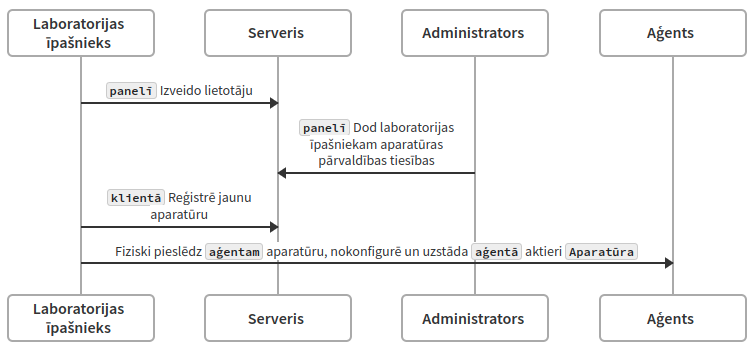
\includegraphics[width=1.0\linewidth]{assets/lab.png}
    \centering
    \caption{Platformas uzstādīšana laboratorijas digitalizācijai.}
    \label{fig:labsetup}
\end{figure}

Lai sajustu, kāda ir lietotāja pieredze, ir vērts novērtēt aģenta uzstādīšanas
komandu \ref{lst:agentconfig}, kas izveido aktieri \lstinline!Aparatura!,
izveido savienojumu ar serveri un veic aparatūras pārvaldību pēc servera
komandām. Minētā komanda informē komandu rindas rīku, ka aparatūra ir Digilent
Anvyl paveida \lstinline!agent-anvyl!, platformā aparatūra ir reģistrēta ar noteiktu
identifikatoru \lstinline!-b ...!, fiziski piesaistītā aparatūra ir ar noteiktiem
konfigurēšanas/programmēšanas parametriem \lstinline!-n ... -s ...! un ka aparatūrai ir
pieejams noteikts seriālās komunikācijas ports \lstinline!-f ...!.

\begin{lstlisting}[caption={Aģenta uzstādīšana komandu rindā},label={lst:agentconfig},captionpos=b]
dip_client agent-anvyl -b 5b17a393-9004-40ec-a9db-e0bb1e77a0e6 -n Anvyl \
    -s 0 -f /dev/serial/by-id/usb-Digilent_...-if01-port0
\end{lstlisting}

Attēlā \ref{fig:development} aprakstīts kā izskatītos izstrādātāja platformas
izmantošana, lai digitāli un attālināti bez tiešas, fiziskas aparatūras
piekļuves veiktu aparatūras programmēšanu, testēšanu un izmantošanu. Kā arī
komandā \ref{lst:quickrun} ir redzams, ka, lai gan programmēšanas mehānisms
pamatā ir sarežģīts, no izstrādātāja skatpunkta aparatūras attālināta
programmēšana un seriālā komunikācija var tikt abstrahēta gana, lai tas šķistu
diezgan intuitīvi. Komandā redzams norādījums izpildīt programmatūras
augšupielādi serverī un aparatūrā, un uzsākt seriālo komunikāciju
\lstinline!quick-run!, aparatūras identifikators platformā \lstinline!-b ...!,
sakompilētas programmaparatūras faila ceļš izstrādātāja datorā \lstinline!-f ...!
un vēlamās izmantojamās \glslink{vinterface}{virtuālās saskarnes} veids
\lstinline!-t ...!.

\begin{lstlisting}[caption={Programmaparatūras augšupielāde un seriālās komunikācijas klienta komanda},label={lst:quickrun},captionpos=b]
dip_client quick-run -b f65e4276-2d72-4471-b5de-bddbc833d2ea \ 
    -f ./main.bit -t minos
\end{lstlisting}

\begin{figure}[H]
    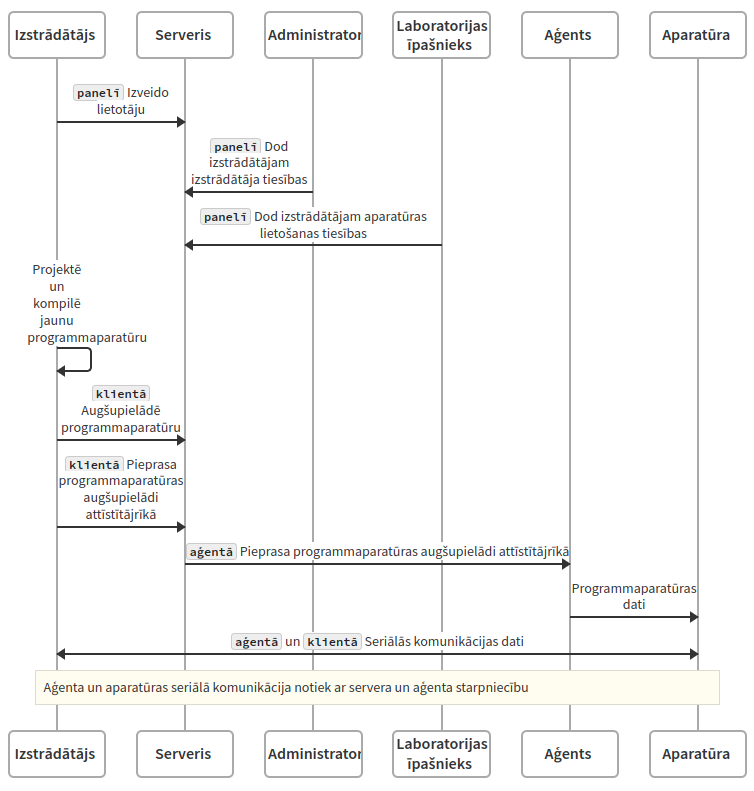
\includegraphics[width=1.0\linewidth]{assets/agent.png}
    \centering
    \caption{Attīstītājrīka aparatūras attālināta programmēšana.}
    \label{fig:development}
\end{figure}

\section{Tīmekļa kameras virtuālā saskarne}
\label{sec:vinweb}

Pēc darba vadītāja ieteikumiem, tika secināts, ka gadījumos, kad attālināta
aparatūras programmēšana nefunkcionē korekti, būtu diezgan grūti bez fiziskas
klātbūtnes secināt, kas ir pie vainas, tādēļ būtu noderīgi, ja būtu pieejama
aparatūras video straumēšana ar tīmekļa kameru.

Lai realizētu šo funkcionalitāti, tika izveidoti dažādi \ref{sec:dipactorsystem}
nodaļā minēti servera un aģenta aktieri, lai veiktu tīmekļakameras datu
starpniecību. Zemāk aprakstīts šo aktieru dzīvescikls un ziņapmaiņa.

\begin{enumerate}
    \item Tīmekļa kameras datu avots ir ar komandu rindas rīku nokonfigurējams
        aktieris \lstinline!agent-video!
    \item \lstinline!agent-video! pievienojas serverim, tādējādi serverī
        izveidojot aktieri \lstinline!server-video-control!, kas sūta atpakaļ
        \lstinline!agent-video! informāciju par straumes abonentu skaitu
    \item \lstinline!agent-video! no fiziski pievienotas tīmekļa kameras saņem
        video straumes datus
    \item Atkarībā no tā vai ir aktuāli video straumes abonenti,
        \lstinline!agent-video! sūta \lstinline!server-video-control! video
        straumes datus, lai ietaupītu patērētos tīkla resursus
    \item Serverī \lstinline!server-video-control! publicē video straumes datus,
        izmantojot aktieri \lstinline!pub-sub!
    \item Pārvaldības panelim pieslēdzas lietotāji, pieprasot video straumi, kas
        rezultē jauna aktiera izveidē \lstinline!server-video-subscriber!, kurš
        informē \lstinline!server-video-control! un \lstinline!pub-sub! par savu
        abonamentu
    \item \lstinline!pub-sub! saņemot video straumes datus no
        \lstinline!server-video-control!, pārtranslē šos datus arī
        \lstinline!server-video-subscriber!
    \item \lstinline!server-video-subscriber! aizsūta lietotājam atpakaļ HTTP
        \lstinline!application/ogg! atbildē aktuālos video straumes datus
\end{enumerate}

\begin{figure}[H]
    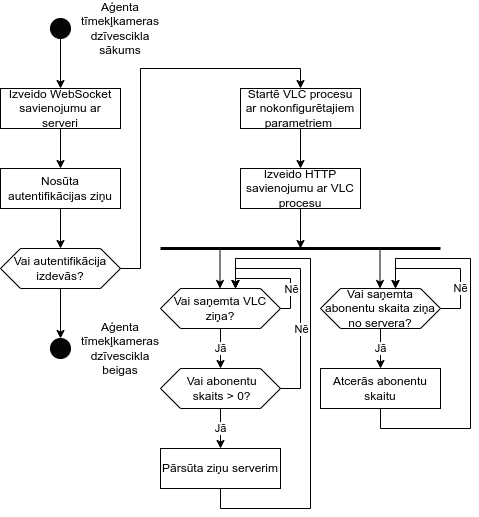
\includegraphics[width=0.6\linewidth]{assets/video_engine.drawio.png}
    \centering
    \caption{Tīmekļa kameras aģenta loģika.}
    \label{fig:videoengine}
\end{figure}

Attēlā \ref{fig:videoengine} ir redzama iepriekšminētā \lstinline!agent-video!
komandu rindas aktiera dzīvescikla loģika. Jāmin, ka brīžos, kad jebkas noiet
greizi, aktieris vienkārši izbeidz visus aktīvos savienojumus un beidz darbu.

Savukārt, attēlos \ref{fig:mgmtpanelhw} un \ref{fig:hwstream} ir redzams
pārvaldības paneļa aparatūras pārvaldības skats, no kura iespējams sākt
skatīties aparatūras video straumi, kā arī piemērs kā izskatās šāda video
straume pārlūkā, precīzāk, kā izskatās publiski pieejamā
\cite{VeinbahsKrisjanisProduction} testa vides laboratorijas video straume, kas
tiek raidīta no darba autora mājām.

\begin{figure}[H]
    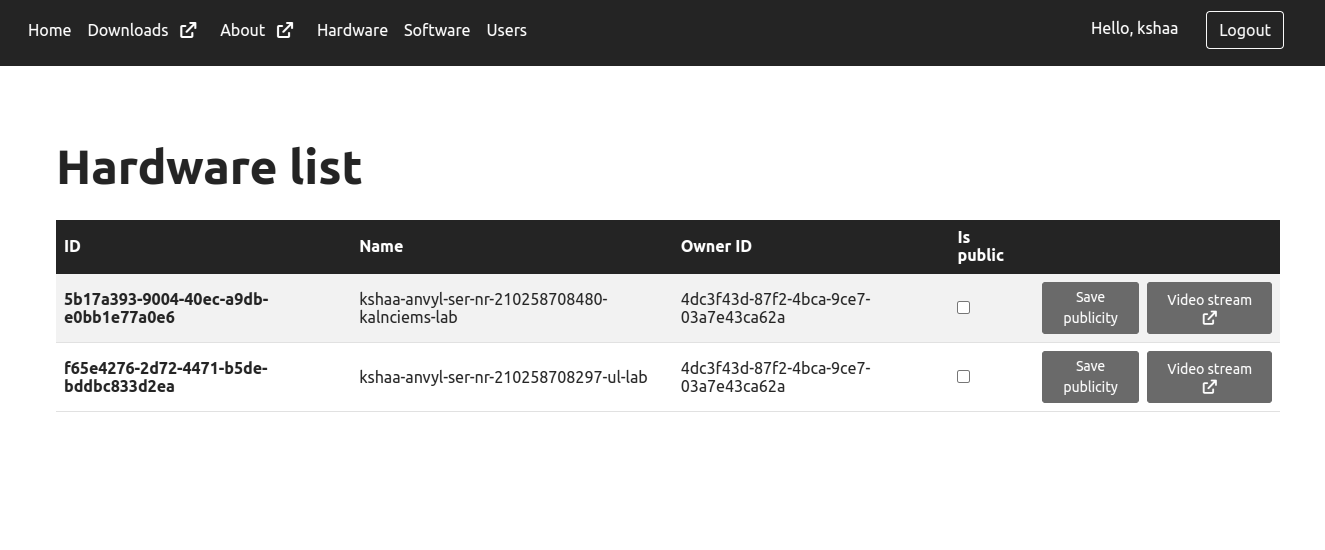
\includegraphics[width=0.9\linewidth]{assets/mgmt-panel-hw-gray.png}
    \centering
    \caption{Platformas pārvaldības paneļa lietotāju pārvaldības skats.}
    \label{fig:mgmtpanelhw}
\end{figure}

\begin{figure}[H]
    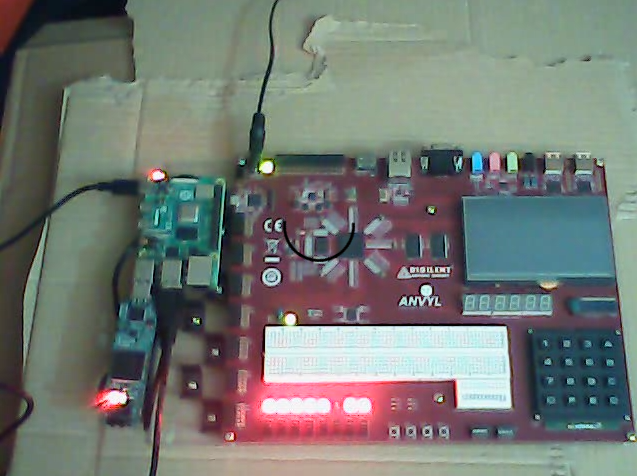
\includegraphics[width=0.9\linewidth]{assets/webcam-usage.png}
    \centering
    \caption{Pārvaldības paneļa aparatūras video straume.}
    \label{fig:hwstream}
\end{figure}

Diemžēl, jāmin, ka augstāk aprakstītajai video straumes translēšanas pieejai ir
pāris tehniskas un veiktspējas problēmas, kas tika atklātas izstrādes un
pētniecības laikā.

Pirmkārt, aģents ir izstrādāts Python programmēšanas valodā, kas nav īsti
paredzēta tādai paralēlai datu apstrādei, kas realizēta tīmekļa kameras datu
straumēšanas aktierī.

Otrkārt, pārtranslēt VLC HTTP OGG straumi varētu nebūt pārāk efektīvi, labāk
būtu izmantot kādu bibliotēku, kas piedāvā šādu funkcionalitāti bez papildus
HTTP savienojuma nepieciešamības.

Treškārt, aģents ir mikrokontrolieris ar vājiem skaitļošanas resursiem, tādēļ
nav ieteicams, nedz pat īsti iespējams, no aģenta raidīt vairāk kā vienu
straumi, kas nozīmē, ka servera pusē to ir jāduplicē ar \gls{pubsub}
mehānismiem, taču tas nebūt nav triviāli, jo video straumes datos ir iekodēta
dienasta informācija par to, kurš aktuālais kadrs šobrīd tiek rādīts, kas,
savukārt, ietekmē to kā serverim ir jāizsūta HTTP OGG atbildes, kas nozīmē, ka
ir jāveic programmatiska video datu lasīšana vai iespējams pat pārrakstīšana.
Precīzāk, sūtot HTTP \lstinline!application/ogg! atbildes daļas, ir nepieciešams
norādīt \lstinline!Range! galveni, kas saturētu informāciju par to kurā video
straumes laikā parādās minētie video dati. \cite[para. 14.35.2]{RFC2616} Šī
informācija ir iekodēta OGG lapās laukā \lstinline!granule_position! \cite[para
6., A]{RFC3533}, taču, lai to nolasītu ir jāizstrādā OGG lapu parseris, ko darba
izstrādes laika ierobežojumu dēļ nebija iespējams laicīgi izdarīt. Darba
ietvaros šim trešajam punktam tika realizēti dažādi aprisinājumi (1. straumes
sākšana no jauna katru reizi, kad ir jauns abonents, 2. straumes pirmo lapu
atcerēšanās un sākotnēja nosūtēšana tādējādi imitējot straumes korektu sākumu,
kam seko pārrāvums līdz aktuālajam brīdim), taču tie nebija pārāk augstas
kvalitātes, kas rezultēja straumes lēnumā un pārrāvumos. 

\section{Baitu virtuālās saskarnes}
\label{sec:vinbytes}

Pats primitīvākais veids kā uzturēt seriālo komunikāciju ir sūtīt starp uz un no
aparatūras baitus. Izmantojot šādu primitīvu komunikācijas mehānismu, lai
lietotājs varētu attālināti mijiedarboties ar aparatūru, ir izstrādātas divas
virtuālas saskarnes, kas realizētas 1) kā termināļa tekstuāla saskarne un 2) kā
termināļa grafiskā saskarne.

Tekstuālā baitu līmeņa termināļa saskarne komandu rindas rīkā tiek dēvēta par
\lstinline!hexbytes!, izmantojot šo tekstuālo saskarni aparatūras lietotājam
jeb, ticamāk, izstrādātājam ir iespējams nolasīt no aparatūras nākošos baitus kā
heksidecimālu simbolu virkni, savukārt, aparatūrā ir iespējams sūtīt baitus
spiežot datora klaviatūras spiedpogas, kas tiek interpretētas kā ASCII simboli,
kuru baitu vērtība tiek sūtīta uz aparatūru. Šādas tekstuālas virtuālās
saskarnes pielietojumu, izmantojot platformas komandu rindas rīku, var skatīt
tekstā \ref{lst:hexbytes}, kur redzama attālināta pieslēgšanās noteiktas
aparatūras (pēc platformā reģistrēta identifikatora) seriālajam portam,
izmantojot virtuālo saskarni \ref{lst:hexbytes}, kas tiek pārtraukta procesam
nododot \lstinline!SIGINT! signālu, izmantojot \lstinline!Ctrl+C! klaviatūras
spiedpogu kombināciju.

\begin{lstlisting}[caption={\lstinline!hexbytes! izmantošana no komandu rindas},label={lst:hexbytes},captionpos=b]
$ dip_client hardware-serial-monitor \
    -b f65e4276-2d72-4471-b5de-bddbc833d2ea -t hexbytes
[0x0] [0x2] [0x2e] [0x0] [0x1] [0x0] [0x6] 
[0x0] [0x0] [0x0] [0x0] [0x0] [0x1] [0x0] [0x6]  
Success: Finished monitoring
\end{lstlisting}

Grafiskā baitu līmeņa termināļa saskarne komandu rindas rīkā tiek dēvēta par
\lstinline!buttonleds!, programmatiski tā funkcionē tāpat kā iepriekšminētā
virtuālā saskarne, jo baiti tiek sūtīti uz aparatūru un baiti tiek saņemti no
aparatūras, taču lietotājam šī mijiedarbība tiek pasniegta izmantojot grafisku
saskarni, kurā ir 24 spiedpogas baitu vērtībā no \lstinline!0x00! līdz
\lstinline!0x17! un 8 LED gaismas 8 bitu jeb baita vērtībā. Šīs virtuālās
saskarnes izsaukums redzams tekstā \ref{lst:buttonleds} un saskarnes izskats
attēlā \ref{fig:buttonleds}.

\begin{lstlisting}[caption={\lstinline!buttonleds! izsaukums no komandu rindas},label={lst:buttonleds},captionpos=b]
$ dip_client hardware-serial-monitor \
    -b f65e4276-2d72-4471-b5de-bddbc833d2ea -t buttonleds
[2022-04-29 21:37:24] [INFO] [monitor_button_led_bytes_app] Starting app
[2022-04-29 21:37:50] [INFO] [monitor_button_led_bytes_app] App finished
Success: Finished monitoring
\end{lstlisting}

\begin{figure}[H]
    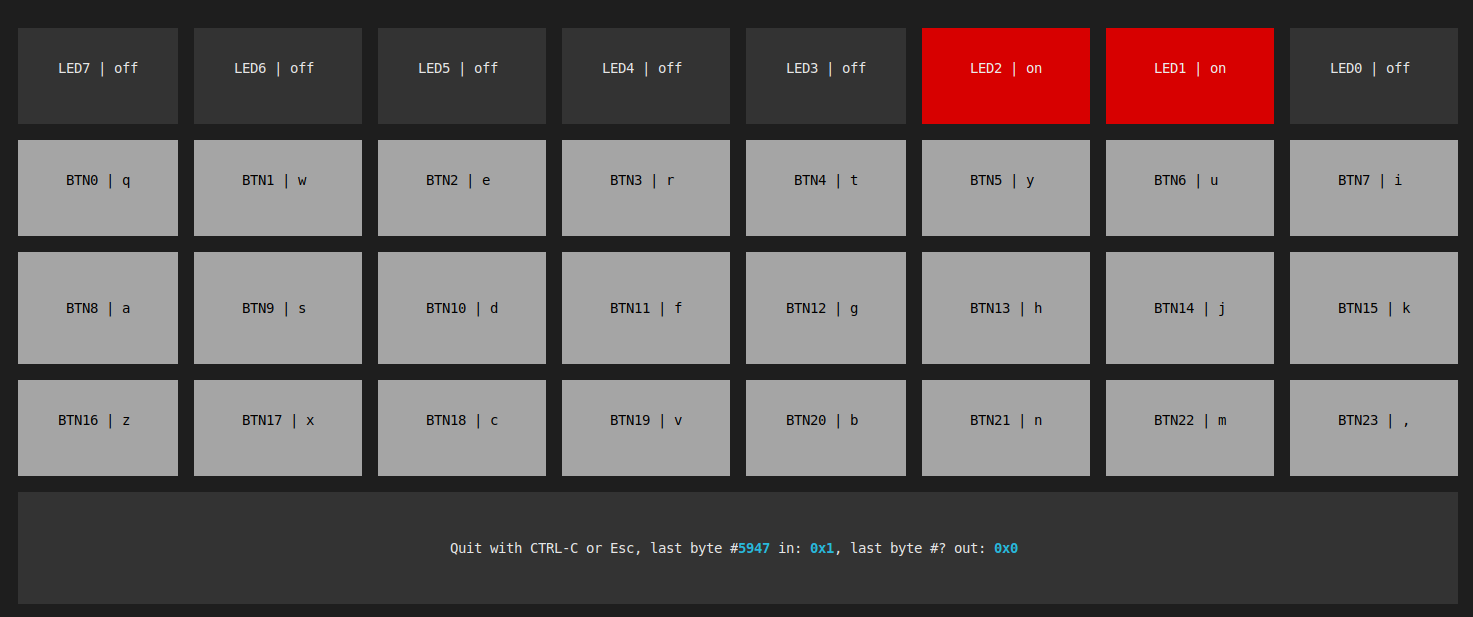
\includegraphics[width=0.9\linewidth]{assets/buttonleds.png}
    \centering
    \caption{\lstinline!buttonleds! virtuālā grafiskā saskarne}
    \label{fig:buttonleds}
\end{figure}

Šādas baitu līmeņa saskarnes jau ir ļoti spējīgas, ar tām var piemēram,
projektēt galīgu stāvokļu automātus vai pat šādus automātus, kas veic darbības
ar papildus reģistru atmiņu. Un spiedpogas var izmantot kā ievaddatus, lai
darbinātu šādu automātu stāvokļu pārejas.

Tomēr šādām saskarnēm ir trūkums - vienā sūtījumā ir pieejams tikai viens baits,
kas patiesībā nav daudz, it īpaši, ja sūtījumā vēlas sūtīt dažāda veida datus.
Ja nu ir nepieciešamība sūtīt 4 slēdžu aktuālos datus un spiedpogu ievaddatus?
Tad izsūtītajā baitā 4 biti jāizmanto slēdžu vērtībām un pārējie 4 spiedpogu
vērtībām. Bet ko darīt, ja jāizsūta 16 slēdžu vērtības? Tad ar baitu vairs
nepietiek, nepieciešami vairāki baiti, tādēļ tika izstrādāta sarežģītāka
virtuālā saskarne MinOS, kas aprakstīta nodaļā \ref{sec:vinminos}.

\section{MinOS virtuālā saskarne}
\label{sec:vinminos}

MinOS ir virtuāla saskarne, lai mijiedarbotos ar attīstītājrīku aparatūru, kas
ir realizēta kā termināļa grafiskā saskarne, kas redzama attēlā
\ref{fig:minosgui} un konceptuāli tā līdzinās tai pašai fiziskai saskarnei, kas
pieejama uz Anvyl attīstītājrīka, kas redzama attēlā \ref{fig:anvyl}. 

Skatoties attēla \ref{fig:minosgui} saskarnē, ir redzams 8x8 RGB displejs (skat.
kreiso daļu), 8 sarkanas LED gaismas (skat. labās puses 1. rindu), 8 sarkani LED
slēdži (skat. labās puses 2. rindu), 3x8 pelēkas spiedpogas (skat. labās puses
3.-5. rindu), teksta lauki (skat. labās puses 6.-7. rindu). 

\begin{figure}[H]
    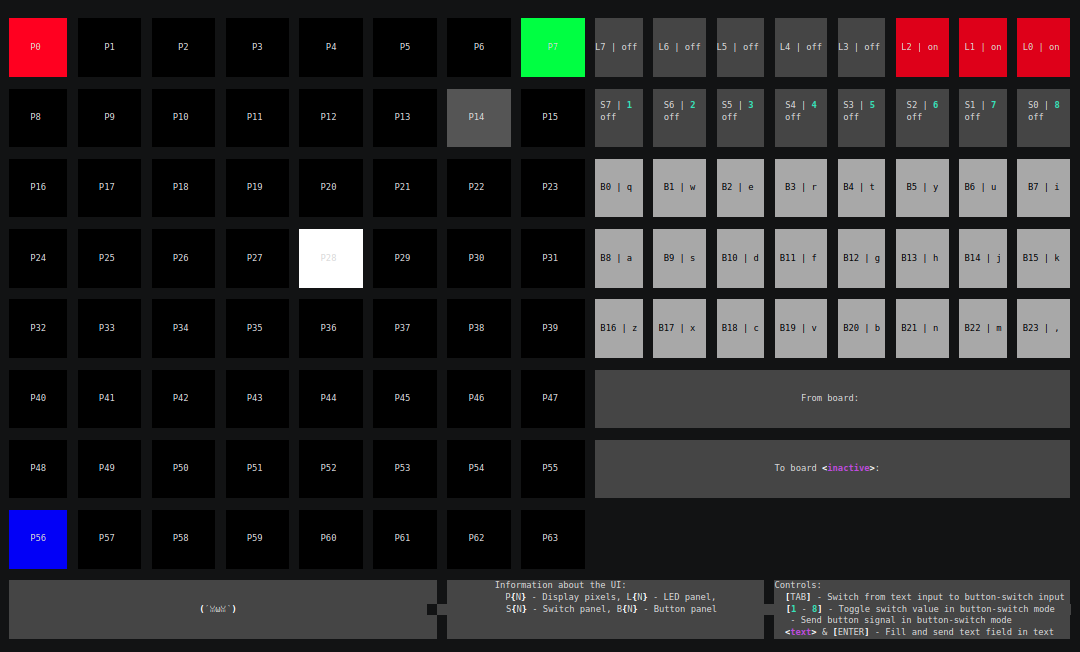
\includegraphics[width=1.0\linewidth]{assets/min-os-execution.png}
    \centering
    \caption{MinOS termināļa grafiskā saskarne.}
    \label{fig:minosgui}
\end{figure}

\begin{figure}[H]
    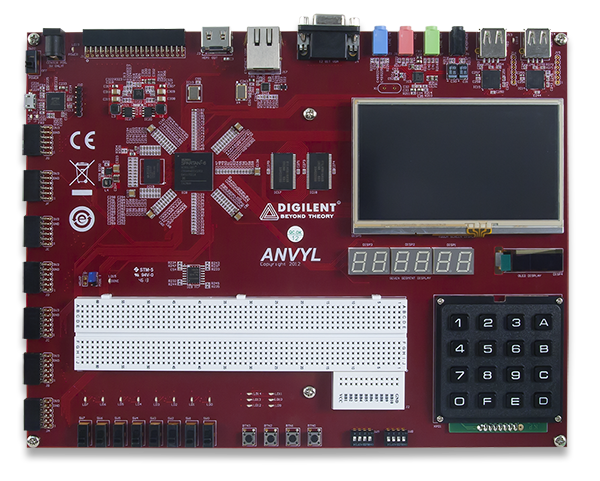
\includegraphics[width=0.7\linewidth]{assets/anvyl.png}
    \centering
    \caption{Anvyl attīstītājrīks.}
    \label{fig:anvyl}
\end{figure}

Lai realizētu MinOS virtuālo saskarni ir nepieciešams uz un no aparatūras sūtīt
dažāda veida datus. Gana daudz, lai ar vienu baitu nepietiktu, jo lai izsūtītu
64 pikseļu RGB displejam pat viena pikseļa datus ir nepieciešami 6 biti krāsai
(\(2^2 * 3\)) un vēl 6 biti indeksam (\(\log_{2}64\)), tātad kopā 12 biti, kas
ir vairāk par 8 bitiem jeb baitu, kas izmantots iepriekšminētās virtuālās
saskarnēs. Un MinOS saskarnē vēlamo elementu ir vairāk nekā tikai RGB displejs,
tādēļ nepieciešams protokols, lai sūtītu vairāku veidu baitu ziņas seriālajā
komunikācijā.

MinOS saskarnes vairāku baitu ziņapmaiņai tika izplānots komunikācijas protokols
starp \glslink{board}{aparatūru} un klientu. Protokols tika formāli definēts,
izstrādājot BNF formāta sintaksi, kuru iespējams apskatīt pielikumā
\ref{att:minosbnf}. Ņemot vērā, ka vēlamais protokols ir binārs, tad BNF formāts
definē baitus kā heksidecimālu ciparu pārus tātad formātā \lstinline!0x??!.

Kā piemērs ziņai, kas atbilst pielikumā pieejamajam BNF formātam ir binārā ziņa
\ref{lst:minosledchunk}, kas MinOS saskarnē tiek izmantota, lai sūtītu LED
gaismas datus no aparatūras uz klientu grafiskai attēlošanai.

\begin{lstlisting}[caption={MinOS LED gaismu pakete},label={lst:minosledchunk},captionpos=b]
    0x00 0x02 0xFF 0x00 0x01 
\end{lstlisting}

MinOS ziņapmaiņas protokols rakstiskā valodā ir sekojošs.
\begin{enumerate}
    \item Baitu straumē var sastapt diva veida simbolus:
    \begin{enumerate}
        \item \lstinline!escaped! simbolus
        \item ne \lstinline!escaped! simbolus
    \end{enumerate}
    \item \lstinline!escaped! simboli ir jebkurš baits, pirms kura iepriekšējais ir baits ir \lstinline!0x00!
    \item Ne \lstinline!escaped! simbols ir tāds, pirms kura iepriekšējais baits nav \lstinline!0x00!
    \item Ja baitu straumē sastopams \lstinline!0x00 0x00!, tad jāpieņem, ka
        sākotnējā \lstinline!escaped! simbola sūtīšana netika korekti pabeigta
        un ir sākusies nākamā \lstinline!escaped! simbola sūtīšana
    \item Ir diva veida \lstinline!escaped! simboli: 
    \begin{enumerate}
        \item Ziņas beigu simbols \lstinline!0x01!
        \item Tipizētas ziņas sākuma simbols \(x\), kur \(x\geq0x02\)
    \end{enumerate}
\end{enumerate}

Ar šādu protokola definīciju ir iespējams sūtīt vairāku baitu ziņas, kur katrai
ziņai piemīt tips, kas ir skaitlis vērtībā no \(0\) līdz \(2^8-2\). Šis
protokols arī ir izmantots MinOS saskarnē, lai sūtītu ziņas no lietotāja
aparatūrai un otrādi. 

Kā piemēru skatoties iepriekšminēto LED gaismas ziņu \ref{lst:minosledchunk}
varam redzēt, ka ziņa sākas ar \lstinline!0x00 0x02!, tātad LED gaismas ziņas
tips ir \(0x02 - 2 = 0x00\) jeb \(0\), redzams, ka ziņa korekti beidzas ar
simbolu \lstinline!0x00 0x01!. Un ziņai pa vidu ir vērtība \lstinline!0xFF!, kas
apzīmē, ka no 8 LED gaismām visas ir ieslēgtas (visi 8 biti ir ar vērtību 1). Ja
šo ziņu pārbauda ar kādu tiešsaistē pieejamu BNF sintakses pārbaudes rīku,
piemēram, BNF playground, \cite{BNFPlayground} pret simbolu \lstinline!<chunk>!,
izmantojot pielikumā definēto protokola sintaksi, kas ir ziņas simbols, tad šī
ziņa veiksmīgi iziet pārbaudi.

Daļa no šāda protokola izstrādes sarežģītības nāk ne tikai no tā plānošanas, bet
arī no tā realizācijas, jo jāatcerās, ka, lai gan realizēt parseri Python
programmēšanas valodā ir triviāli, realizēt to Verilog programmaparatūrā ir
mazliet grūtāk.

Attēlā \ref{fig:chunkparser} redzams galīgs determinēts stāvokļu automāts, kas
realizē pielikumā pieejamās BNF sintakses parsēšanu, nolasot ziņas tipu un
datus. Gadījumos, kad ievaddati neatbilst nevienai pārejai, automāts paliek tajā
pašā stāvoklī, kurā jau šobrīd atrodās. Attēlā redzamās pārejas pirmajā rindā
satur pārejas ievaddatu nosacījumus un otrā rindā, pārejas blakusefektus jeb
izpildītās darbības. Šis automāts nav pilnīgs, jo patiesībā ir nepieciešami
papildus dienasta dati, lai glabātu aktuālo parsētās ziņas indeksu datu buferī,
taču šī loģika netika ielikta ilustrācijā, lai to pārāk nesarežģītu. Šādu
automātu ir iespējams vienkārši realizēt gan Verilog valodā, gan Python valodā,
kas arī tika darīts, lai realizētu MinOS virtuālo saskarni.

Automātā pieminētie ievaddati ir ielasītā baita gatavība
\lstinline!is_rx_ready!, ielasītā baita vērtība \lstinline!rx_data!. Automātā
pieminētie izvaddati ir ziņas veids \lstinline!r_chunk_type! un ziņas datu
buferis \lstinline!r_chunk_bytes!. Automātā pieminēta arī palīgvērtība - ziņas
aktuālā baita indekss buferī \lstinline!buffer_index!.

\begin{figure}[H]
    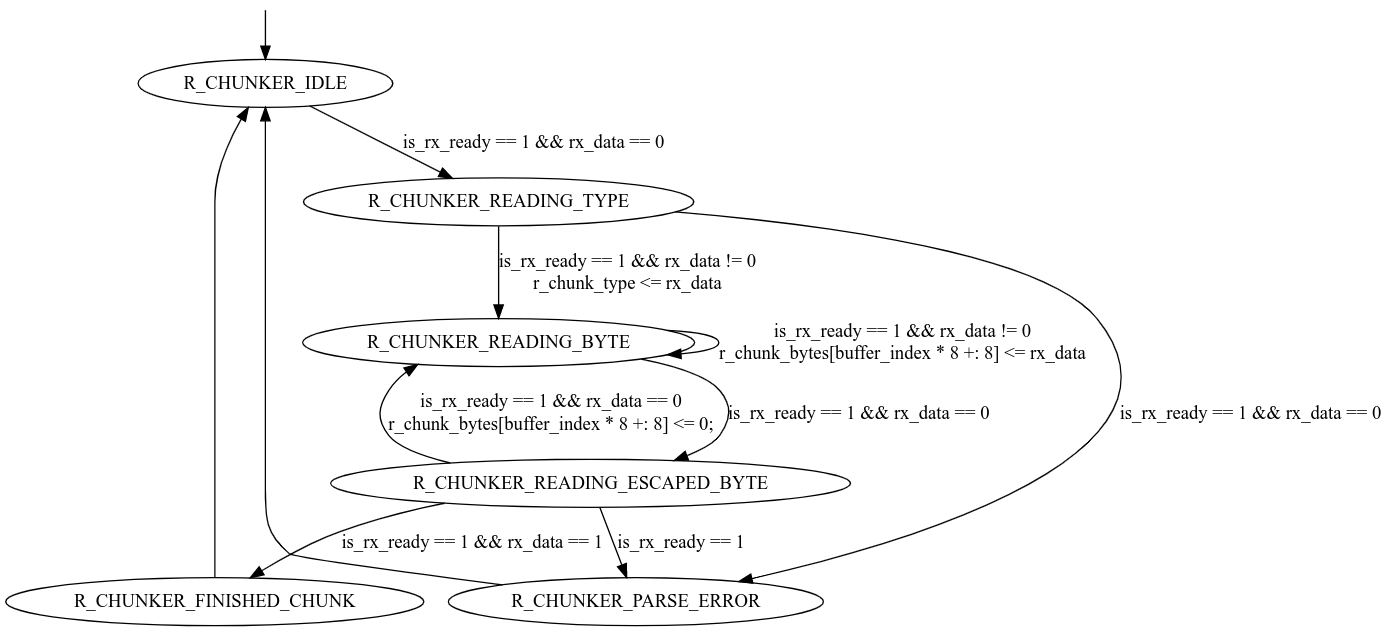
\includegraphics[width=1.0\linewidth]{assets/chunkparser.png}
    \centering
    \caption{MinOS ziņu parsera galīgs determinēts automāts.}
    \label{fig:chunkparser}
\end{figure}

Lai gan lejupielādējot platformas klienta komandu rindas rīku uzreiz ir pieejama
Python valodā programmētā grafiskā saskarne, tomēr attīstītājrīkā ir
nepieciešama atbilstoša programmaparatūra, kas komunicē izmantojot MinOS
protokolu, tādēļ projekta ietvaros Verilog valodā tika izstrādāts MinOS modulis,
kas abstrahē seriālo komunikāciju un izstrādātājam izvērš tikai interesējošos
virtuālās saskarnes elementus. Attēlā \ref{fig:minos} redzama šī Verilog moduļa
grafiskā interpretācija. 

\begin{figure}[H]
    
\includegraphics[width=0.7\linewidth]{assets/min-os-grey.png}
    \centering
    \caption{MinOS programmaparatūras modulis.}
    \label{fig:minos}
\end{figure}

Attēlā \ref{fig:minos} redzamais Verilog valodā izstrādātais modulis izvērš
dažādus signālus, lai mijiedarbotos ar attālināto grafisko lietotāja MinOS
saskarni. Tabulā \ref{table:minossignals} ir dokumentēti no moduļa izvērstie
signāli un to būtība.

\begin{table}[H]
    \newcounter{minossignalcounter}
    \newcommand\rownumber{\stepcounter{minossignalcounter}\arabic{minossignalcounter}.}
    \begin{tabular}{ |p{1cm}|p{3cm}|p{2cm}|p{3cm}|p{6cm}| }
    \hline
    N.p.k.&Signāls&Virziens&Izmērs&Būtība \\
    \hline
    \rownumber&\lstinline!CLK!&I&1&Pulksteņa signāls \\
    \hline
    \rownumber&\lstinline!T19!&I&1&Seriālā porta ievaddatu signāls \\
    \hline
    \rownumber&\lstinline!display!&I&\(64 * 8 = 512\)&Displeja pikseļu krāsas datu signāls \\
    \hline
    \rownumber&\lstinline!leds!&I&8&LED gaismu signāli \\
    \hline
    \rownumber&\lstinline!tx_text_bytes!&I&\(32 * 8 = 256\)&Izsūtītā ASCII teksta datu signāls \\
    \hline
    \rownumber&\lstinline!tx_text_size!&I&8&Izsūtītā ASCII teksta izmēra signāls \\
    \hline
    \rownumber&\lstinline!T20!&O&1&Seriālā porta izvaddatu signāls \\
    \hline
    \rownumber&\lstinline!button_index!&O&1&Nospiestās spiedpogas indeksa signāls \\
    \hline
    \rownumber&\lstinline!button_pressed!&O&1&Spiedpogas nospiešanas stāvokļa signāls \\
    \hline
    \rownumber&\lstinline!rx_is_text_ready!&O&1&Iesūtītā ASCII teksta gatavības signāls \\
    \hline
    \rownumber&\lstinline!rx_text_bytes!&O&\(32 * 8 = 256\)&Iesūtītā ASCII teksta datu signāls \\
    \hline
    \rownumber&\lstinline!rx_text_size!&O&8&Iesūtītā ASCII teksta izmēra signāls \\
    \hline
    \rownumber&\lstinline!switches!&O&8&Slēdžu stāvokļu signāls \\
    \hline
    \end{tabular}
    \centering
    \captionsetup{justification=centering}
    \caption{Verilog MinOS moduļa signāli, I - ievad signāls, O - izvadsignāls}
    \label{table:minossignals}
\end{table}

Ar šādu virtuālu saskarni un tās Verilog realizāciju jau ir iespējams projektēt
daudz sarežģītākas digitālas iekārtas. Tehniski, ņemot vērā, ka ir pieejams 64
RGB krāsu monitors un spiedpogas, būtu jābūt iespējai ar šādu abstrakciju
attālināti projektēt, testēt un spēlēt datorspēli "Tetris" tikpat ārti kā esot
fiziski klāt attīstītājrīku aparatūrai, kas ir cienījams sasniegums!

Būtu vērtīgi līdz galam definēt ziņas, kādas atbalsta MinOS saskarne. Kā jau
iepriekš ilustrēts, MinOS saskarne atbalsta sūtīt ziņu par LED gaismu stāvokli.
Visas MinOS atbalstītās ziņas, savukārt, aprakstītas tabulā \ref{table:minospackets}.

\begin{table}[H]
    \newcounter{minospacketcounter}
    \newcommand\rownumber{\stepcounter{minospacketcounter}\arabic{minospacketcounter}.}
    \begin{tabular}{ |p{1cm}|p{3cm}|p{2cm}|p{8cm}| }
    \hline
    N.p.k.&Nosaukums&Izmērs&Būtība \\
    \hline
    \rownumber&\lstinline!leds!&1 baits&8 LED gaismu stāvoklis \\
    \hline
    \rownumber&\lstinline!switches!&1 baits&8 slēdžu stāvoklis \\
    \hline
    \rownumber&\lstinline!buttons!&1 baits&\(2^8\) spiedpogu nospiešanas fakts \\
    \hline
    \rownumber&\lstinline!display!&2 baiti&6 biti pikseļa indeksam, 6 biti pikseļa RGB krāsu vērtībām \\
    \hline
    \rownumber&\lstinline!text!&32 baiti&ASCII teksta vērtība \\
    \hline
    \end{tabular}
    \centering
    \captionsetup{justification=centering}
    \caption{MinOS virtuālās saskarnes atbalstītās ziņas}
    \label{table:minospackets}
\end{table}

\section{Infrastruktūras pārvaldība}
\label{sec:ops}

Kā laboratorijas īpašnieki pieslēdz savus dzelžus platformai?

Kā klienti pieslēdzas sistēmai un gūst iespēju izmantot dzelžus?

Kā izstrādātājs jeb darba autors jeb es automatizē versionēšanu, artefaktu pārvaldību?

Docker cross-platform w/ buildx i.e. buildkit

Board management w/ Ansible

CICD deployment procesi

\section{Testēšana un uzturēšana}
\label{sec:usage}

Šo es praktiski neesmu paspējis izdarīt, bet šis būtu interesanti:

Waveform recordings

WASM testing

Ko reāli varētu izdarīt (drīzumā uzkodēšu, šim vajadzētu būt ātri):

MinOS request and response
